% METRIC SPACES NOTES
% OLIVER DIXON, 2023

% TODO: Remaining lectures:
%   IX
%   X
%   XI
%   XII
%   XIII
%   XIV
%   XV

% Video camera vector graphic adapted under CC0 from SVGRepo:
% https://www.svgrepo.com/svg/475018/video-call

\documentclass{article}

\usepackage[
    a4paper,
    top=1.5in,
    bottom=1.5in,
    left=1in,
    right=1in,
]{geometry}
\usepackage[
    angle=90,
    hanchor=l,
    hpos=.05\paperwidth,
    fontsize=1.5em,
    color=black,
    firstpageonly,
]{draftwatermark}
\usepackage[en-GB]{datetime2}
\usepackage[missing=master]{gitinfo2}
\usepackage{fancyhdr, anyfontsize, amsthm, mathtools, amssymb, tcolorbox,
    tocloft, titlesec, lastpage, enumitem, tikz, multirow}
\usepackage[hypcap=false]{caption}
\usepackage[
    colorlinks,
    allcolors=blue,
]{hyperref}
\usepackage[nameinlink]{cleveref}

% BEGIN DOCUMENT METADATA

\title{Metric Spaces}
\author{Oliver Dixon}
\date{Semester I, 2023/24}
\newcommand*\internalname{metric-spaces}
\newcommand*\modulecode{MAT00051I}

% END DOCUMENT METADATA

\newcommand*\githublink{https://github.com/oliverdixon/l5-notes/}
\newcommand*\subtitle{Consolidated Lecture Notes}
\urlstyle{same}
\newcommand*\fclower[2]{\relax\lowercase{#1}#2}
\renewcommand*\vec{\mathbf}
\DraftwatermarkOptions{text={Warning: Incomplete notes; do not redistribute.
    Check for \href{\githublink}{GitHub updates} periodically.}}

\setlength\parskip{.8em}
\setlength\parindent{0pt}
\setlength\cftparskip{0pt}
\renewcommand*\baselinestretch{1.2}
\captionsetup[figure]{justification=centering}

\definecolor{ballfill}{RGB}{242, 242, 242}
\usetikzlibrary{decorations.pathreplacing, calc, shapes.geometric, arrows.meta}
\tikzset{
    every node/.style={transform shape},
    unitaxes/.pic={
        \draw[->] (-1.5, 0)--(1.5, 0) node[right] {$x$};
        \draw[ultra thick] (-1, -.1) -- (-1, .1);
        \draw[ultra thick] (1, -.1) -- (1, .1);
        \draw[->] (0, -1.5)--(0, 1.5) node[above] {$y$};
        \draw[ultra thick] (-.1, 1) -- (.1, 1);
        \draw[ultra thick] (-.1, -1) -- (.1, -1);
    },
    squarespace/.pic={
        \draw plot[smooth cycle, tension=0.8] coordinates {(2,2)
            (1.5,0) (2,-2) (0,-1.5) (-2,-2) (-1.5,0) (-2,2) (0,1.5)};
    },
    longspace/.pic={
        \draw plot[smooth cycle, tension=0.8] coordinates {(5,1)
            (5,0) (5,-1) (0,-2) (-5,-1) (-5,0) (-5,1) (0,2)};
    },
}

\newcommand*\iffforward{\par\boxed\Longrightarrow\ }
\newcommand*\iffbackward{\par\boxed\Longleftarrow\ }

\tcbuselibrary{theorems, breakable, skins}
\tcbset{
    enhanced,
    parbox=false,
    before upper=\hspace{-3.5pt},
    colback=white, colbacktitle=white, coltitle=black,
    fonttitle=\bfseries,
    rounded corners=all,
    toptitle=1ex, bottomtitle=1ex, top=2ex, bottom=2ex,
    titlerule=1pt,
    description font=\normalfont,
    separator sign none,
    breakable,
    fontlower=\slshape,
}

% \newtheoremtype: create a new tcolorbox theorem-like environment which will be
% included as a subsection in the table of contents.
%
%   #1: display name (e.g. Definition)
%   #2: environment name (e.g. definition)
%   #3: colour of the bounding box, according to xcolor (e.g. red)
%
% NOTE: Creating an auxiliary environment is slightly circuitous, but the
% '/tcb/new/list inside' and '/tcb/list entry' keys are not (currently)
% sufficiently general to handle complex table-of-contents constructions such as
% the one required here.
%
\makeatletter
\newcommand*\newtheoremtype[3]{
    \newtcbtheorem[auto counter, number within=section, Crefname={#1}{#1s},
        crefname={\fclower{#1}\relax}{\fclower{#1}\relax s}]
        {aux:#2}{#1}{colframe=#3}{#2}
    \NewDocumentEnvironment{#2}{m+m}{
        \expandafter\csname aux:#2\endcsname{##1}{##2}
        \addcontentsline{toc}{subsection}{#1 \ref*{#2:##2}: ##1}
        \ignorespaces
    }{\expandafter\csname endaux:#2\endcsname}
}
\makeatother

\titleformat\section[runin]{\scshape \LARGE}{}{0pt}{}[\hfill \mbox{}]
\makeatletter
\renewcommand*\cftsecpresnum{\begin{lrbox}{\@tempboxa}}
\makeatother
\renewcommand*\cftsecaftersnum{\end{lrbox}}
\setlength\cftsecnumwidth{0pt}
\renewcommand*\contentsname{Lecture Contents}
\renewcommand*\cfttoctitlefont{\scshape \LARGE \hfill}
\renewcommand*\cftaftertoctitle{\hfill \mbox{}}

% \lecture: start a new lecture section, with a description and Panopto link.
%
%   #1: lecture display name
%   #2: Panopto video/folder URL suffix (or empty if no recording)
%   #3: lecture summary paragraph
%   #4: date of live delivery
%
\newcommand\lecture[4]{
    \section{#1}\hfill
    \raisebox{3pt}{
        \ifstrempty{#2}{
            \textit{No recording}\hspace*{8pt}
            \fbox{\centering\includegraphics[width=13pt]{../icons/no-video.pdf}}
        }{
            \textit{#4}\hspace*{8pt}
            \href{https://york.cloud.panopto.eu/Panopto/Pages/#2}
                {\fbox{\centering\includegraphics[width=13pt]%
                    {../icons/video.pdf}}}
        }%
    }%
    \par #3
    \vskip.5\baselineskip
}

\newtheoremtype{Definition}{definition}{black}
\newtheoremtype{Example}{example}{blue}
\newtheoremtype{Theorem}{theorem}{red}

\newcommand*\crefrangeconjunction{~to~}
\creflabelformat{equation}{#2#1#3}
\crefname{equation}{equation}{equations}
\Crefname{equation}{Equation}{Equations}
\numberwithin{equation}{section}

\Crefname{figure}{Figure}{Figures}
\crefname{figure}{figure}{figures}
\numberwithin{figure}{section}

\setlist{itemindent=1em}
\newlist{axioms}{enumerate}{1}
\crefname{axiomsi}{axiom}{axioms}
\Crefname{axiomsi}{Axiom}{Axioms}
\newcommand*\setaxiomprefix[1]{
    \setlist[axioms]{label=#1\arabic*), ref=#1\arabic*}
}

\renewcommand*\thesection{\Roman{section}}
\let\Sectionmark\sectionmark
\def\sectionmark#1{\def\sectionname{#1}\Sectionmark{#1}}
\renewcommand*\headrulewidth{0pt}
\renewcommand*\footrulewidth{\headrulewidth}
\makeatletter
\fancypagestyle{mainbody}{
	\fancyhf{}
    \fancyhead[L]{\itshape \@title: \subtitle}
    \fancyhead[R]{\itshape \@date}
    \fancyfoot[L]{\itshape \@author}
    \fancyfoot[R]{\itshape Page \thepage\ of \pageref*{LastPage}}
}
\makeatother

\begin{document}
\thispagestyle{empty}
\pagestyle{plain}
\pagenumbering{roman}
\begin{titlepage}
    \begin{flushright}
        \makeatletter
        \begingroup
            \fontsize{50}{50}\selectfont
            \slshape \sffamily \@title
            \LARGE
            \vskip\baselineskip
            \subtitle
        \endgroup
        \vfill
        \begingroup
            \Large \obeylines
            \setlength\parskip{.5em}
            Collated and Typeset by \@author
            Based on the %
            \href{https://www.york.ac.uk/students/studying/manage/%
                programmes/module-catalogue/module/\modulecode/}{\modulecode} %
            Lecture Series
            \vskip\baselineskip
            University of York
            \@date
        \endgroup
        \makeatother
    \end{flushright}
    \vfill
    \begin{center}
        \begin{tabular}{r|l}
            Compilation Date & \today \\
            Author Contact & \href{mailto: Oliver Dixon <od641@york.ac.uk>}%
                {od641@york.ac.uk} \\
            Sources Link & \url{\githublink tree/\gitBranch/\internalname} \\
            Latest Commit Hash & \href{\githublink commit/\gitHash}{\gitHash}
                (\gitBranch) \\
            York Web Link & \url{https://www-users.york.ac.uk/~od641/l5-notes/%
                \internalname .pdf} \\
            Document Licence & \href{\githublink blob/\gitBranch/LICENSE}
                {MIT Licence} (all rights reserved on draft copies)
        \end{tabular}
    \end{center}
\end{titlepage}
\stepcounter{page}
\tableofcontents
% \vfill
% \begin{center}
%     \setlength\fboxsep{6pt}
%     \footnotesize \fbox{Dedicated to Maia}
% \end{center}
\clearpage
\pagenumbering{arabic}
\pagestyle{mainbody}

\lecture{Lecture I}{Viewer.aspx?id=c3a52a78-486e-4e1d-88fc-b083009b9766}{
    Lecture One introduces the concept of a \emph{metric} as a generalisation of
    the notion of distance between two points in a set. Three \emph{canonical
    metrics} on $\mathbb{R}^N$ are presented; these are then generalised
    further, and a short proof verifies the compliance of the generalised
    Euclidean metric with the relevant axioms.
}{\DTMdisplaydate{2023}{09}{26}{Tuesday}}

\begin{definition}{Metric Space}{metric}
    Suppose that $ X $ is a set, and $ d \colon X \times X \to [0, \infty)
    \subset \mathbb{R} $. Then, $ d $ is a \emph{metric} on $ X $ if and only if
    the following properties hold for $ a, b, c \in X $:
    \setaxiomprefix{M}
    \begin{axioms}
        \item \emph{Positivity.} $ d(a, b) \geq 0 $;
        \item \emph{Equality.} $ d(a, b) = 0 \iff a = b $;
        \item \emph{Symmetry.} $ d(a, b) = d(b, a) $;
        \item \emph{Triangularity.} $ d(a, b) \leq d(a, c) + d(b, c) $
            \label{axiom:triangle-inequality}.
    \end{axioms}
    The tuple $ (X, d) $ is a \emph{metric space}.
\end{definition}
\begin{definition}{Canonical Metrics on \texorpdfstring{$\mathbb{R}^N$}{an
        N-dimensional real vector space}}{canon-metrics}
    We can consider three metrics on $ \mathbb{R}^N $: $ d_1 $, $ d_2 $, and
    $ d_\infty $, each of which have a domain of $ \mathbb{R}^N \times
    \mathbb{R}^N $ and a codomain of $ [0, \infty) $:
    \begin{align}
        d_1(\vec{x}, \vec{y}) &= \sum_{i=1}^N \vert \vec{x}_i - \vec{y}_i
            \vert\label{eqn:d1-metric} \\
        d_2(\vec{x}, \vec{y}) &= \left[\sum_{i=1}^N (\vec{x}_i - \vec{y}_i)^2
            \right]^{1/2} \label{eqn:d2-metric} \\[.8em]
        d_\infty(\vec{x}, \vec{y}) &= \max_{1 \leq i \leq N} \vert \vec{x}_i -
            \vec{y}_i \vert\label{eqn:dinf-metric}
    \end{align}
    Unless otherwise stated, $ \mathbb{R}^N $ is endowed with $ d_2 $ Euclidean
    metric. This is consistent with our current understanding of the real line,
    which uses the absolute value $ \vert x - y \vert $ to denote distance
    between $ x, y \in \mathbb{R} $.
\end{definition}
\begin{example}{Unit Circles in the Three Canonical Spaces}{unit-circles}
    Using the definitions of the canonical metrics \cref{eqn:d1-metric},
    \cref{eqn:d2-metric}, and \cref{eqn:dinf-metric} (and a very loose
    understanding of a \emph{circle}) we can draw the unit ``circles'' generated
    in $ \mathbb{R}^2 $ under each of these metrics. For instance,
    \cref{fig:dinf-unit-circle} shows the boundary of the set $ S^2_\infty $,
    where
    \begin{equation}
        S^2_\infty = \left\{ (x, y) \in \mathbb{R}^2 \colon d_\infty(x, y) \leq
        1 \right\}.
    \end{equation}

    \begin{minipage}{.3\linewidth}
        \centering
        \begin{tikzpicture}
            \pic at (0, 0) {unitaxes};
            \node[diamond, draw, minimum width=2cm, minimum height=2cm] {};
        \end{tikzpicture}
        \captionof{figure}{Unit Circle in $ d_1 $}%
        \label{fig:d1-unit-circle}
    \end{minipage}\hfill
    \begin{minipage}{.3\linewidth}
        \centering
        \begin{tikzpicture}
            \pic at (0, 0) {unitaxes};
            \draw (0, 0) circle[radius=1];
        \end{tikzpicture}
        \captionof{figure}{Unit Circle in $ d_2 $}%
        \label{fig:d2-unit-circle}
    \end{minipage}\hfill
    \begin{minipage}{.3\linewidth}
        \centering
        \begin{tikzpicture}
            \pic at (0, 0) {unitaxes};
            \draw (-1, 1) -- (1, 1) -- (1, -1) -- (-1, -1) -- (-1, 1);
        \end{tikzpicture}
        \captionof{figure}{Unit Circle in $ d_\infty $}%
        \label{fig:dinf-unit-circle}
    \end{minipage}
\end{example}
\begin{theorem}{The Generalised Metric is a Metric}{general-dp-metric}
    Consider the $ d_p $ metric, where $ d_p \colon \mathbb{R}^N \times
    \mathbb{R}^N \to [0, \infty) $ is a generalisation of the $ d_2 $ Euclidean
    metric for $ p \in \mathbb{N} $:
    \begin{equation}
        (\vec{x}, \vec{y}) \mapsto \left[\sum_{i=1}^N \vert \vec{x}_i -
        \vec{y}_i \vert^p\right]^{1/p} \label{eqn:dp-metric} \text { for all }
        \vec{x}, \vec{y} \in \mathbb{R}^N.
    \end{equation}
    Then, $ (\mathbb{R}^N, d_p) $ is a metric space.
    \begin{proof}
        To show that $ d_p $ is a metric on $ \mathbb{R}^N $, we must verify
        that $ d_p $ is in compliance with the constraints enumerated in
        \cref{definition:metric}. The positivity, equality, and symmetry axioms
        are easy to show, so we will focus on the triangularity property here,
        proving it by demonstrating a reduction to \emph{Minkowski's Theorem}.

        Let $ \vec{a}_k $ and $ \vec{b}_k $ be such that
        \begin{align}
            d_p(\vec{x}, \vec{z}) &\eqcolon \left[\sum_{k=1}^N \vert \vec{a}_k
                \vert^p\right]^{1/p} \\
            d_p(\vec{y}, \vec{z}) &\eqcolon \left[\sum_{k=1}^N \vert \vec{b}_k
                \vert^p\right]^{1/p}.
        \end{align}
        Then, note that $ d_p(\vec{x}, \vec{y}) $ (as defined in
        \cref{eqn:dp-metric}) can be
        written in terms of $ \vec{a}_k $ and $ \vec{b}_k $, since $ \vec{a}_k =
        \vec{x}_k - \vec{z}_k $ and $ \vec{b}_k = \vec{y}_k - \vec{z}_k $ for
        $ k = 1, \ldots, N $:
        \begin{equation}
            d_p(\vec{x}, \vec{y}) = \left[\sum_{k=1}^N \vert \vec{a}_k +
            \vec{b}_k \vert^p\right]^{1/p}.
        \end{equation}
        The triangle inequality, as stated in \cref{axiom:triangle-inequality},
        requires that
        \begin{equation}
            \left[\sum_{k=1}^N \vert \vec{a}_k + \vec{b}_k \vert^p\right]^{1/p}
            \leq \left[\sum_{k=1}^N \vert \vec{a}_k \vert^p\right]^{1/p} +
            \left[\sum_{k=1}^N \vert \vec{b}_k \vert^p\right]^{1/p}.
        \end{equation}
        This inequality is equivalent to the well-known Minkowski's Theorem;
        thus, $ d_p $ satisfies the triangle inequality over $ \vec{x}, \vec{y},
        \vec{z} \in \mathbb{R}^N $.
    \end{proof}
\end{theorem}

\lecture{Lecture II}{Viewer.aspx?id=e35adcae-8b46-4472-8b19-b085009bdfe1}{
    Lecture Two introduces the concept of the \emph{supremum} and \emph{infimum}
    as properties of any subset of the reals. The sets of \emph{bounded} and
    \emph{continous} functions are introduced as $ B([0, 1]) $ and $ C([0, 1]) $
    respectively, and we prove that the ``sup-metric'' $ d_\infty $ forms a
    metric on $ B([0, 1]) $.
}{\DTMdisplaydate{2023}{09}{28}{Thursday}}

\begin{definition}{Supremum and Infimum}{sup-inf}
    If $ S \subset \mathbb{R} $ is a set, then $ \sup S $ is defined to be the
    \emph{least upper bound} of $ S $. This is defined to be the smallest $ b
    \in \mathbb{R} $ such that $ x \leq b $ for all $ x \in S $. The infimum of
    $ S $, $ \inf S $, is defined analogously as the \emph{greatest lower
    bound}.

    \centering
    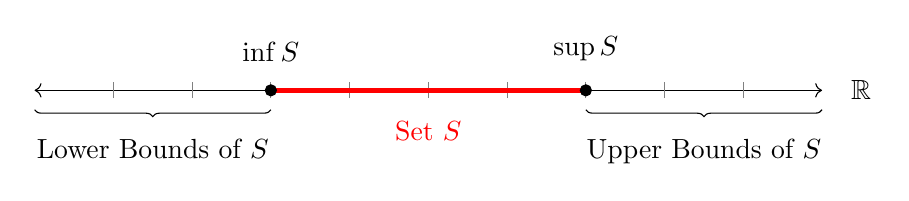
\begin{tikzpicture}
        \coordinate (setstart) at (-2, 0);
        \coordinate (setend) at (2, 0);
        \draw[<->] (-5, 0) -- (5, 0) node[right, xshift=7pt] {$ \mathbb{R} $};
        \draw[decoration={brace, mirror, raise=7pt}, decorate] (-5, 0) --
            (setstart) node[pos=0.5, anchor=north, yshift=-14pt]
            {Lower Bounds of $ S $};
        \draw[decoration={brace, mirror, raise=7pt}, decorate] (setend) --
            (5, 0) node[pos=0.5, anchor=north, yshift=-14pt]
            {Upper Bounds of $ S $};
        \foreach \i in {-4, ..., 4} \draw[gray] (\i, -.1) -- (\i, .1);
        \draw[ultra thick, red] (setstart) -- (setend) node[pos=0.5,
            anchor=north, yshift=-7pt]{Set $ S $};
        \filldraw (setstart) circle (2pt) node[above, yshift=7pt] {$ \inf S $};
        \filldraw (setend) circle (2pt) node[above, yshift=7pt] {$ \sup S $};
    \end{tikzpicture}
    \captionof{figure}{$ S \subset \mathbb{R} $  and its bounding points on the
        real line}
\end{definition}
\begin{definition}{The \texorpdfstring{$ \ell^\infty $}{Ell-Infinity}
        Set of Bounded Sequences}{ell-infinity}
    Consider $ \mathbb{R}^\mathbb{N} $: the set of all sequences of reals. We
    cannot work with this entire space, since many real sequences are unbounded,
    and the $ d_1 $ and $ d_2 $ canonical metrics give rise to non-finite sums.
    Therefore, we consider the set $ \ell^\infty $ as the \emph{set of
    all bounded real sequences}:
    \begin{equation}
        X \in \ell^\infty \iff \exists M > 0 \text{ such that }
            \vert X_n \vert \leq M \text { for all } n \in \mathbb{N}.
    \end{equation}
    Then, the infinity metric is defined in terms of the supremum, since a
    sequence with infinite terms mightn't possess a maximum:
    \begin{equation}
        d_\infty(X, Y) = \sup\left\{\vert X_i - Y_i \vert \colon
            i \in \mathbb{N}\right\} \text { for } X, Y \in \ell^\infty.
    \end{equation}
\end{definition}
\begin{definition}{The Set of Bounded Functions}{bounded-functions-set}
    $ B([0,1]) $ is the \emph{set of all bounded functions} $ f $ such that
    $ f \colon [0, 1] \to \mathbb{R} $.
\end{definition}
\begin{definition}{The Set of Continuous Functions}{cts-functions-set}
    $ C([0,1]) $ is the \emph{set of all continuous functions} $ f $ such that
    $ f \colon [0, 1] \to \mathbb{R} $.
\end{definition}
\begin{theorem}{The set of bounded functions\texorpdfstring{ over $[0, 1]$}{}
    with the sup-metric forms a metric space}{bounded-is-metric}
    Consider the $ d_\infty $ metric on $ B([0, 1]) $ defined in terms of the
    supremum, such that the upper bound needn't lie in the set:
    \begin{equation}
        d_\infty \colon B([0, 1]) \times B([0, 1]) \to [0, \infty)
            \text{ such that } (f, g) \mapsto \sup\left\{\vert f(t) - g(t) \vert
            \colon t \in [0, 1] \right\}.
    \end{equation}
    Then, $ \left(B([0, 1]),\, d_\infty\right) $ is a metric space.
    \begin{proof}
        We must verify that $ d_\infty : B([0, 1]) \times B([0, 1]) \to [0,
        \infty) $ satisfies the metric axioms described in
        \cref{definition:metric} for all $ f, g, h \in B([0, 1]) $.
        \begin{itemize}
            \item Since $ f-g $ is a bounded function, there exists an $ M \geq
                0 $ for which $ f(t) - g(t) \leq M $ for all $ t \in [0, 1] $.
                Thus, $ \sup\left\{\vert f(t) - g(t) \vert \colon t \in [0,
                1]\right\} \geq 0 $, and $ d_\infty(f, g) \geq 0 $ for all $ f,
                g \in B([0, 1]) $.
            \item \iffforward If $ f = g $, then $ \vert f(t) - g(t) \vert = 0 $
                for all $ t \in [0, 1] $, so $ d_\infty(f, g) = \sup\{0, 0,
                \ldots\} = 0 $.

                \iffbackward Furthermore, if $ d_\infty(f, g) = 0 $, then we
                know that $ \sup\left\{ \vert f(t) - g(t) \vert \colon t \in [0,
                1] \right\} = 0 $. We know that $ \vert f(t) - g(t) \vert \geq 0
                $, so $ \vert f(t) - g(t) \vert = 0 $ follows immediately, from
                which we can conclude that $ f(t) = g(t) $ for all $ t \in [0,
                1] $, hence $ f = g $.

                Thus, $ d_\infty(f, g) = 0 \iff f = g $.
            \item By the symmetry of the standard metric on $ \mathbb{R} $, the
                symmetry of $ d_\infty $ on $ B([0, 1]) $ follows immediately:
                \begin{align}
                    d_\infty(f, g) &= \sup\left\{ \vert f(t) - g(t) \vert \colon
                        t \in [0, 1] \right\} \\
                    &= \sup\left\{ \vert g(t) - f(t) \vert \colon t \in [0, 1]
                        \right\} \\
                    &= d_\infty(g, f).
                \end{align}
            \item By the triangularity property of the standard metric on $
                    \mathbb{R} $,
                \begin{align}
                    d_\infty(f, g) &= \sup\left\{ \vert f(t) - g(t) \vert \colon
                        t \in [0, 1] \right\} \\
                    &= \sup\left\{ \vert f(t) - h(t) + h(t) - g(t) \vert \colon
                        t \in [0, 1] \right\} \\
                    &\leq \sup\left\{ \vert f(t) - h(t) \vert \colon t \in [0,
                        1] \right\} + \sup\left\{ \vert h(t) - g(t) \vert \colon
                        t \in [0, 1] \right\} \\
                    &= d_\infty(f, h) + d_\infty(h, g),
                \end{align}
                hence $ d_\infty $ possesses the property of triangularity on $
                B([0, 1]) $.
        \end{itemize}
        Thus, $ \left(B([0,1]), d_\infty\right) $ is a metric space.
    \end{proof}
\end{theorem}

\lecture{Lecture III}{Viewer.aspx?id=afbe7e12-8494-4fe3-b73f-b08a009bdc46}{
    Lecture Three opens with a counterexample to challenge a common
    misconception. It continues to introduce the concept of \emph{norms} as
    generalisations of the absolute value function, \emph{metric subspaces}, and
    \emph{isometric maps}, complemented by a simple example.
}{\DTMdisplaydate{2023}{10}{03}{Tuesday}}

\begin{example}{Binary Strings}{binary-strings}
    Despite the examples seen thus far, metric spaces needn't support an
    associated arithmetic or algebraic structure. For instance, let $ \Sigma =
    \{ 0, 1 \}^\mathbb{N} $ be the set of binary strings (sequences of zeroes
    and ones). If $ \sigma = \left(a_n\right)_{n=1}^\infty \in \Sigma $ and $
    \sigma^\prime = \left(b_n\right)_{n=1}^\infty \in \Sigma $, consider the
    distance function $ d \colon \Sigma \times \Sigma \to [0, \infty) $ such
    that
    \begin{equation}
        \left(\sigma, \sigma^\prime\right) \mapsto
        \begin{cases}
            0 &\text{ if } a_n = b_n \quad \forall n \in \mathbb{N}; \\
            1/\min\left\{n \colon a_n \neq b_n\right\} &\text{ otherwise.} \\
        \end{cases}.
    \end{equation}
    Despite there being no inherent algebraic structure or ordering on $ \Sigma
    $, $ d $ is a metric that is inversely proportional with the earliest point
    at which two given binary strings diverge, thus providing a notion of
    \emph{distance}.
    \tcblower
    This example was adapted from Ben Green's University of Oxford
    \href{https://courses.maths.ox.ac.uk/course/view.php?id=65}{Metric Spaces
    and Complex Analysis} Michaelmas 2021 course notes.
\end{example}
\begin{definition}{Norm}{norm}
    A \emph{norm} is an abstraction of the absolute value. Suppose that $ V $ is
    a normable vector space. Then $ \vert\vert\cdot\vert\vert \colon V \to
    \mathbb{R} $ is such that, for all $ \vec{x}, \vec{y} \in V $,
    \setaxiomprefix{N}
    \begin{axioms}
        \item $ \vert\vert \vec{x} \vert\vert \geq 0 $;
        \item $ \vert\vert \vec{x} \vert\vert = 0 \iff \vec{x} = \vec{0} $;
        \item $ \vert\vert \lambda \vec{x} \vert\vert = \vert \lambda \vert
            \vert\vert \vec{x} \vert\vert $ for all $ \lambda \in \mathbb{R} $;
        \item $ \vert\vert \vec{x} + \vec{y} \vert\vert \leq \vert\vert \vec{x}
            \vert\vert + \vert\vert \vec{y} \vert\vert $.
    \end{axioms}
    $ V $ equipped with $ \vert\vert \cdot \vert\vert $ is a \emph{normed
    space}. Note that any norm can give rise to a metric; such a metric is
    sometimes called the \emph{metric induced by the norm}.
\end{definition}
\begin{definition}{Metric Subspace}{metric-subspace}
    Suppose that $ (X, d) $ and $ (Y, e) $ are metric spaces. We say that $ X $
    is a \emph{metric subspace} of $ Y $ if $ X \subseteq Y $ and $ d $ is a
    restriction of $ e $ to $ X \times X $.
\end{definition}
\begin{definition}{Isometric Map}{isometric-map}
    Suppose that $ (X, d) $ and $ (Y, e) $ are metric spaces, and that $ \phi
    \colon X \to Y $ is surjective. Then $ \phi $ is called an \emph{isometric
    map} if and only if $ e(\phi(a), \phi(b)) = d(a, b) $ for all $ a, b \in X
    $. This will later be used to define the most rigid definition of
    ``sameness'' for metric spaces.
\end{definition}
\begin{example}{Complex Isometry}{complex-isometry}
    Each $ (a, b) \in \mathbb{R} $ is associated with a unique $ z = a +
    \mathrm{i}b \in \mathbb{C} $ such that $ \Re(z) = a $ and $ \Im(z) = b $.
    Notice that $ (a, b) \mapsto a + \mathrm{i}b $ is a bijective map from $
    \mathbb{R}^2 $ to $ \mathbb{C} $, and hence qualifies as an isometry.
\end{example}

\lecture{Lecture IV}{Viewer.aspx?id=3a47174e-ed9d-413d-b309-b08c009bdb8e}{
    Lecture Four begins an investigation into the topology of a metric space. In
    particular, we introduce \emph{open and closed balls}, \emph{interior
    points}, \emph{boundary points}, and \emph{exterior points}, and define
    \emph{open} and \emph{closed} sets in terms of these concepts. We take an
    example metric space and rigorously compute its interior, boundary, and
    exterior, and finally show (by example) that considering objects as either
    subsets or subspaces can vastly alter their topological properties.
}{\DTMdisplaydate{2023}{10}{05}{Thursday}}

\begin{definition}{Open and Closed Balls}{balls}
    Suppose that $ (X, d) $ is a metric space, and that $ x_0 \in X $. For every
    $ \epsilon > 0 $, we define the \emph{open ball centered at $ x_0 $ with
    radius $ \epsilon $} to be the set $ B(x_0, \epsilon) = \left\{ x \in X
    \colon d(x, x_0) < \epsilon \right\} $. Analogously, the \emph{closed ball
    centered at $ x_0 $ with radius $ \epsilon $} is defined to be the set
    $ \overline{B}(x_0, \epsilon) = \left\{ x \in X \colon d(x, x_0) \leq
    \epsilon \right\} $.

    \centering
    \begin{minipage}{.5\linewidth}
        \centering
        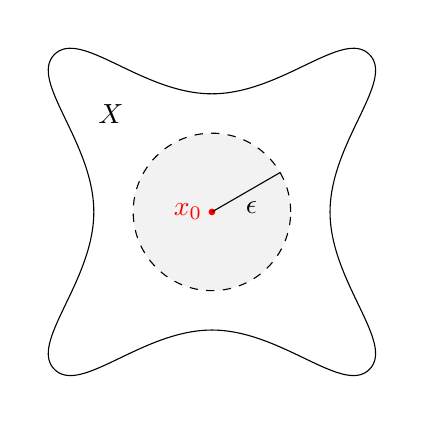
\begin{tikzpicture}
            \pic at (0, 0) {squarespace};
            \draw[fill=ballfill, dashed] (0, 0) circle[radius=1] node[above
                left=1cm]{$ X $};
            \filldraw[red] (0, 0) circle (1pt) node[left] {$ x_0 $};
            \draw (0, 0) -- ++(30:1cm) node[anchor=north, pos=0.5, xshift=2pt]
                {$ \epsilon $};
        \end{tikzpicture}
        \captionof{figure}{The open ball $ B(x_0, \epsilon) \subset X $}
    \end{minipage}\hfill
    \begin{minipage}{.5\linewidth}
        \centering
        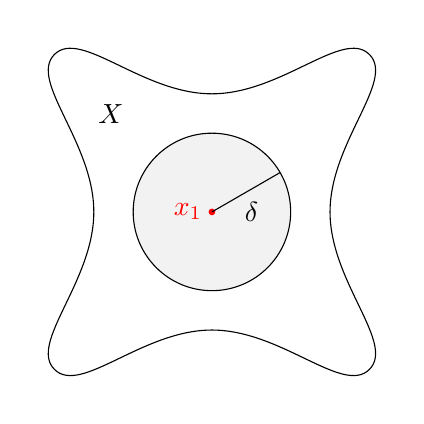
\begin{tikzpicture}
            \pic at (0, 0) {squarespace};
            \draw[fill=ballfill] (0, 0) circle[radius=1] node[above left=1cm]
                {$ X $};
            \filldraw[red] (0, 0) circle (1pt) node[left] {$ x_1 $};
            \draw (0, 0) -- ++(30:1cm) node[anchor=north, pos=0.5, xshift=2pt]
                {$ \delta $};
        \end{tikzpicture}
        \captionof{figure}{The closed ball $ \overline{B}(x_1, \delta)
            \subset X $}
    \end{minipage}
\end{definition}
\begin{definition}{Interior Points}{interior-points}
    Let $ A \subset X $. An \emph{interior point} $ y \in X $ of $ A $ is an
    element for which $ B(y, \epsilon) \subset A $ for some $ \epsilon > 0 $.
    That is, there is an open ball centred at $ y $ with radius $ \epsilon $
    that is completely contained within $ A $. The set of all such points is
    denoted as $ A^o $, and is called \emph{the interior of $ A $}.
\end{definition}
\begin{definition}{Boundary Points}{boundary-points}
    The element $ y \in X $ is a \emph{boundary point} of $ A $ if and only if
    for any $ \epsilon > 0 $, $ B(y, \epsilon) \cap A \neq \emptyset $ and
    $ B(y, \epsilon) \cap A^c \neq \emptyset $. That is, any open ball centred
    at $ y $ always intersects with $ A $ and its complement $ A^c $. The set of
    all such points is denoted as $ \partial A $, and is called \emph{the
    boundary of $ A $}.
\end{definition}
\begin{definition}{Exterior Points}{exterior-points}
    The element $ y \in X $ is an \emph{exterior point} of A if and only if for
    some $ \epsilon > 0 $, $ B(y, \epsilon) \subset A^c $. That is, there exists
    an open ball centred at $ y $ which intersects only with the complement of
    $ A $; this can also be interpreted as an interior point of the complement.
    The set of all such points is denoted as $ A^e $, and is called \emph{the
    exterior of A}.
\end{definition}
\begin{example}{Illustration of Interior, Boundary, and Exterior Points}
        {int-bound-ext-graphic}
    Consider an ambient space $ X $, and the shaded subset $ A \subseteq X $.
    We can illustrate examples of points from the interior, boundary, and
    exterior of $ A $.

    \begin{minipage}{.3\linewidth}
        \centering
        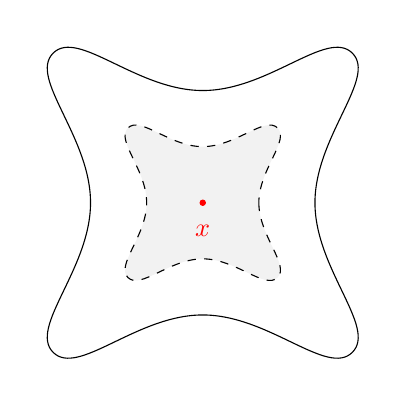
\begin{tikzpicture}[scale=0.95]
            \pic at (0, 0) {squarespace};
            \pic[scale=0.5, every path/.style={fill=ballfill, dashed}] at (0, 0)
                {squarespace};
            \filldraw[red] (0, 0) circle (1pt) node[below, yshift=-5pt] {$ x $};
        \end{tikzpicture}
        \captionof{figure}{An interior point $ x \in A^o $}
    \end{minipage}\hfill
    \begin{minipage}{.3\linewidth}
        \centering
        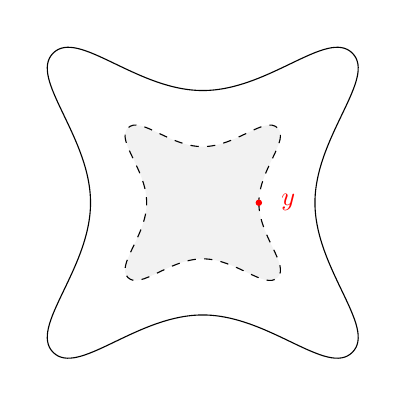
\begin{tikzpicture}[scale=0.95]
            \pic at (0, 0) {squarespace};
            \pic[scale=0.5, every path/.style={fill=ballfill, dashed}] at (0, 0)
                {squarespace};
            \filldraw[red] (.75, 0) circle (1pt) node[right, xshift=5pt]
                {$ y $};
        \end{tikzpicture}
        \captionof{figure}{A boundary point $ y \in \partial A $}
    \end{minipage}\hfill
    \begin{minipage}{.3\linewidth}
        \centering
        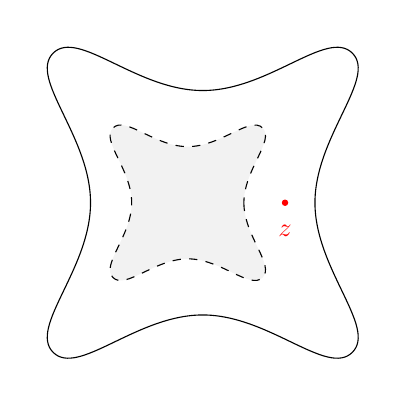
\begin{tikzpicture}[scale=0.95]
            \pic at (.2, 0) {squarespace};
            \pic[scale=0.5, every path/.style={fill=ballfill, dashed}] at (0, 0)
                {squarespace};
            \filldraw[red] (1.3, 0) circle (1pt) node[below, yshift=-5pt]
                {$ z $};
        \end{tikzpicture}
        \captionof{figure}{An exterior point $ z \in A^e $}
    \end{minipage}

    Note that the interior, boundary, and exterior are mutually disjoint and can
    be placed under the disjoint union operation to form the entire ambient
    space. This fact is henceforth denoted by ``$ A^o \coprod \partial A \coprod
    A^e = X $'' for $ A \subseteq X $.
\end{example}
\begin{example}{Finding the interior, boundary, and exterior of a
        set}{int-bound-ext}
    Consider $ (\mathbb{R}, d) $ with $ A = (0, 1] \subset \mathbb{R} $.
    Intuitively, we can conjecture that $ A^o = (0, 1) $, $ \partial A = \{0,
    1\} $, and $ A^e = \mathbb{R} \setminus (0, 1) = (-\infty, 0) \cup (1,
    \infty) $, however these claims must be proven rigorously by (a) showing
    that the conjectured points do belong to the relevant set, and (b) showing
    that the conjectured points are the only elements to belong to the relevant
    set.
    \begin{itemize}
        \item First consider the interior. Take $ x \in (0, 1) $. By
            \cref{definition:interior-points}, we want to show that there is an
            $ \epsilon > 0 $ such that $ B(x, \epsilon) \subset (0, 1] = A $.
            Set $ \epsilon_1 \coloneq x $, and $ \epsilon_2 \coloneq 1-x $.
            Given that $ 0 < x < 1 $, we can take an $ \epsilon \coloneq
            \min\{ \epsilon_1, \epsilon_2 \} $. Then, since $ \epsilon/2 <
            \epsilon_1, \epsilon_2 $,
            \begin{equation}
                B(x, \epsilon/2) = \left\{ y \in \mathbb{R} \colon d(x, y) <
                    \epsilon/2 \right\} \subset A.
            \end{equation}
            This proves that $ (0, 1) \subseteq A^o $.

            We now need to eliminate the remaining candidates in $ \mathbb{R}
            \setminus (0, 1) $ from having possible membership in $ A^o $. The
            points $ x < 0 $ and $ x > 1 $ can be discarded immediately, since
            any open ball centred at these points could never lie totally within
            $ A $, due to their positive radii $ \epsilon $. Finally, we need to
            show that $ \{0,1\} \not\subset A^o $. Without loss of generality,
            pick $ x = 1 $, and take an $ \epsilon > 0 $ to consider the open
            ball $ B(x, \epsilon) $. Any such ball would contain a point that is
            strictly greater than 1, and hence would contain points outside of $
            A $. Thus, $ x \not\in A^o $, and $ A^o = (0, 1) $ as claimed.
        \item Now consider the boundary, as described in
            \cref{definition:boundary-points}. We claim that $ \{0, 1\} =
            \partial A $, and first demonstrate that $ \{0, 1\} \subseteq
            \partial A $.  Without loss of generality, we show that $ 0 \in
            \partial A $. Let $ \epsilon > 0 $, and consider $ B(0, \epsilon) =
            (-\epsilon, \epsilon) $. Clearly, since $ \epsilon > 0 $, $
            (-\epsilon, \epsilon) \cap A \neq \emptyset $ and $ (-\epsilon,
            \epsilon) \cap A^c \neq \emptyset $; thus, $ 0 $ is a boundary
            point.

            Now, we show that there are no other boundary points of $ A $ in $
            \mathbb{R} $. We know that $ \mathbb{R} = A^o \coprod \partial A
            \coprod A^e $, hence $ A^o \cup \partial A = \emptyset $, thus $ (0,
            1) \not\subset \partial A $. Without loss of generality for $ x < 0
            $, consider points $ x > 1 $. Therefore, there exists an $ \epsilon
            > 0 $ such that $ x = 1 + \epsilon $. Considering $ B(x, \epsilon/2)
            $, we can see that $ B(x, \epsilon/2) \subset A^c $, which implies
            that $ B(x, \epsilon/2) \cap A = \emptyset $. Thus, $ \{ 0, 1 \} =
            \partial A $.
        \item Finally, consider the exterior, as described in
            \cref{definition:exterior-points}. Recall that the entire space can
            be expressed as a disjoint union, e.g. $ \mathbb{R} = A^o \coprod
            A^e \coprod \partial A $. Hence,
            \begin{align}
                A^e &= \mathbb{R} \setminus \left( A^o \cup \partial A
                    \right) \\
                &= \mathbb{R} \setminus [0, 1] \\
                &= (-\infty, 0) \cup (1, \infty),
            \end{align}
            as conjectured.
    \end{itemize}
\end{example}
\begin{definition}{Open, Closed, and Clopen Sets}{open-closed-clopen-sets}
    Let $ (X, d) $ be a metric space. A subset $ A $ of $ X $ is \emph{open} if
    and only if $ A \cap \partial A = \emptyset $. A subset $ F $ of $ X $ is
    \emph{closed} if and only if $ \partial F \subseteq F $. Note that a set can
    be both open and closed: typical examples are the empty set and the entire
    space; these sets are called \emph{clopen}.

    \centering
    \begin{minipage}{.5\linewidth}
        \centering
        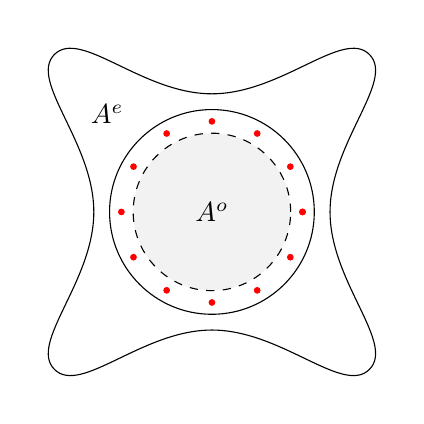
\begin{tikzpicture}
            \pic at (0, 0) {squarespace};
            \draw[fill=ballfill, dashed] (0, 0) circle[radius=1];
            \draw (0, 0) circle[radius=1.3] node {$ A^o $} node[above left=1cm]
                {$ A^e $};
            \foreach \angle in {0, 30, ..., 360}
                \filldraw[red] (\angle:1.15cm) circle (1pt);
        \end{tikzpicture}
        \captionof{figure}{An open set $ A $ does not contain its boundary
            points.}
    \end{minipage}\hfill
    \begin{minipage}{.5\linewidth}
        \centering
        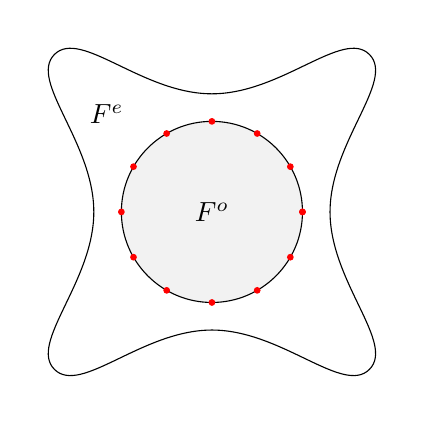
\begin{tikzpicture}
            \pic at (0, 0) {squarespace};
            \draw[fill=ballfill] (0, 0) circle[radius=1.15] node {$ F^o $}
                node[above left=1cm] {$ F^e $};
            \foreach \angle in {0, 30, ..., 360}
                \filldraw[red] (\angle:1.15cm) circle (1pt);
        \end{tikzpicture}
        \captionof{figure}{A closed set $ F $ contains its boundary points.}
    \end{minipage}
\end{definition}
\begin{example}{Subset vs. Subspace}{subset-subspace}
    Consider $ (\mathbb{R}, d) $ with $ A = (0, 1) \cup (1, 2) $. If $ A $ is
    considered as a \emph{subset} if $ \mathbb{R} $, then $ \partial A = \{0, 1,
    2 \} $. Hence, $ A \cap \partial A = \emptyset $, and $ A $ is open by
    \cref{definition:open-closed-clopen-sets}.  Further, $ A $ is not closed,
    since $ \partial A \not\subseteq A $.

    If $ A $ is considered as a \emph{subspace} of $ \mathbb{R} $, then $
    \partial A = \emptyset $, since $ \{ 0, 1, 2 \} \not\subseteq A $, and we
    cannot consider the points outside of the subspace when determining its
    topology. Hence, $ A $ is closed. But $ A \cap \partial A = \emptyset $,
    since $ \partial A = \emptyset $; thus $ A $ is also open, and is ultimately
    clopen when interpreted as a subspace.
\end{example}

\lecture{Lecture V}{Viewer.aspx?id=dbcb156d-d828-454f-929d-b091009bf65b}{
    Lecture Five proves multiple important theorems: a set is open if and only
    if its complement is closed; a set is open if and only if we can place an
    open ball around every point and stay inside of the set; and an open set can
    be expressed as a union of open balls. We also introduce the notion of
    \emph{a topology} $ T_d $ as the collection of all open subsets, and prove
    theorems related to closure under the familiar union and intersection set
    operations.
}{\DTMdisplaydate{2023}{10}{10}{Tuesday}}

\begin{theorem}{A subset is open if and only if its complement is
        closed}{open-subset-closed-complement}
    Consider a set $ A \subseteq X $. Then, $ A $ is open if and only if $ A^c $
    is closed.
    \begin{proof}
        This can be proven by unravelling the definitions of open and closed
        sets (\cref{definition:open-closed-clopen-sets}) and boundary points
        (\cref{definition:boundary-points}).

        \iffforward First, suppose that $ A $ is open.  If $ A = \emptyset $,
        then $ A^c = X $. The entire space is known to be clopen, and thus
        closed. If $ A \neq \emptyset $, then $ A \cap \partial A = \emptyset $,
        and $ \partial A \subseteq A^c $.  We can now see a useful equality by
        using the fact that $ \left(A^c\right)^c = A $:
        \begin{align}
            \partial \left(A^c\right) &= \left\{ y \in X \colon \forall \epsilon
                > 0 \, B(y, \epsilon) \cap A^c \neq \emptyset \land B(x,
                \epsilon) \cap \left(A^c\right)^c \neq \emptyset \right\}%
                \label{eqn:boundary-complement-boundary-first}\\
            &= \left\{ y \in X \colon \forall \epsilon > 0 \, B(y, \epsilon)
                \cap A^c \neq \emptyset \land B(x, \epsilon) \cap A \neq
                \emptyset \right\} \\
            &= \partial A.\label{eqn:boundary-complement-boundary-last}
        \end{align}
        Since $ \partial A \subseteq A^c $, and $ \partial A = \partial
        \left(A^c\right) $, we know that $ \partial \left(A^c\right) \subseteq
        A^c $. Hence, $ A^c $ is closed.

        \iffbackward Next, assume that $ A^c $ is closed, hence $ \partial
        \left(A^c\right) \subseteq A^c $. Given that $ \partial A = \partial
        \left(A^c\right) $, $ \partial A \subseteq A^c $. Since $ A^c \cap A =
        \emptyset $, we know that $ \partial A \cap A = \emptyset $, and thus $
        A $ is open.
    \end{proof}
\end{theorem}
\begin{definition}{The topology of a metric space}{topology}
    The \emph{topology} of a metric space $ (X, d) $ is denoted as $ T_d $, and
    is defined to be \emph{the collection of all open subsets of $ X $}. Note
    that since $ T_d \subseteq \mathcal{P}(X) $, for any set $ X $, $ \emptyset,
    X \in T_d $, so $ T_d \neq \emptyset $.
\end{definition}
\begin{theorem}{Equivalence between openness and the existence of open balls}
        {openness-open-balls}
    Let $ A \subseteq X $ be open. Then, every point of $ A $ is an interior
    point of A. Equivalently, $ A $ is open if and only if there is an open ball
    around every point in $ A $ that resides within $ A $:
    \begin{equation}
        \forall x \in A\, \exists \epsilon > 0 \text{ such that } B (x,
        \epsilon) \subseteq A.
    \end{equation}

    \begin{minipage}{\dimexpr.6\linewidth-2em}
        \begin{proof}
            \iffforward First assume that $ A $ is open. By definition, $ A \cap
            \partial A = \emptyset $. If $ A = \emptyset $, then there exists no
            points to select, and the universal quantifier cannot select any
            points for $ x $. If $ A \neq \emptyset $, then there must be at
            least one $ \epsilon > 0 $ such that $ B(x, \epsilon) \subseteq A $
            or $ B(x, \epsilon) \subseteq A^c $ for any $ x \in A $. But, since
            $ x \in A $, it is not possible that $ B(x, \epsilon) $ is entirely
            contained within $ A^c $, since $ x \in B(x, \epsilon) $. Hence, $
            B(x, \epsilon) \subseteq A^c $, as required.

            \iffbackward Next, suppose that $ \forall x \in A\, \exists \epsilon
            > 0 $ such that $ B (x, \epsilon) \subseteq A $. Take any $ x \in A
            $.  Immediately, we can see that $ x \not\in \partial A $, since $
            B(x, \epsilon) \cap A^c = \emptyset $, because $ B(x, \epsilon)
            \subseteq A $. Hence, $ A $ is open.
        \end{proof}
    \end{minipage}\hfill
    \begin{minipage}{.4\linewidth}
        \centering
        \begin{tikzpicture}
            \coordinate (x1point) at (1, 1);
            \coordinate (x2point) at (-1, 1);
            \coordinate (x3point) at (0, -1);
            \draw[dashed] (0, 0) circle (2.7cm);
            \foreach \pt in {1, 2, 3}{
                \filldraw[red] (x\pt point) circle (1pt);
                \draw[dashed, red] (x\pt point) circle (.4cm*\pt+.05cm)
                    node[below] {$ x_\pt $};
                \draw[red] (x\pt point) -- ++(45*\pt:.4cm*\pt+.05cm);
            }
        \end{tikzpicture}
        \captionof{figure}{Every point supports an open ball}
    \end{minipage}
\end{theorem}
\begin{theorem}{The open ball is open}{open-ball-open}
    For any $ x \in X $ and any $ \epsilon > 0 $, $ B(x, \epsilon) \in T_d $.
    Since $ T_d $ is defined to be a collection of open sets, this statement is
    equivalent to the claim that ``\emph{the open ball is open}''.
    \begin{proof}
        Take an $ x \in X $ and construct the open ball $ B(x, \epsilon) $, for
        a fixed $ \epsilon > 0 $. Take $ y \in B(x, \epsilon) $ and let $ \Delta
        \coloneq d(x, y) $. If $ x=y $, then $ B(x, \epsilon) = B(y, \epsilon)
        \subseteq B(x, \epsilon) $, there is nothing to do; therefore, we assume
        that $ x \neq y $, thus $ \Delta > 0 $ and $ 0 < \Delta < \epsilon $.
        Let $ \epsilon^\prime \coloneq \min\left\{ \Delta, \epsilon-\Delta
        \right\} $ and consider $ B(y, \epsilon^\prime/2) $.

        \begin{minipage}{.45\linewidth}
            To show the openness of the open ball, it is sufficient to show that
            $ B(y, \epsilon^\prime/2) \subseteq B(x, \epsilon) $. By the
            triangle inequality on $ d $, for any $ z \in B(y,
            \epsilon^\prime/2) $,
            \begin{align}
                d(x, z) &\leq d(x, y) + d(y, z) \\
                &\leq \Delta + \epsilon^\prime/2 \\
                &= \Delta + \min\left\{\Delta, \epsilon-\Delta\right\}/2 \\
                &\leq \Delta + (\epsilon-\Delta)/2 \\
                &< \Delta + \epsilon - \Delta \\
                &= \epsilon
            \end{align}
        \end{minipage}\hfill
        \begin{minipage}{.5\linewidth}
            \centering
            \begin{tikzpicture}
                \coordinate (xpoint) at (0, 0);
                \coordinate (ypoint) at (0, 1.5);
                \draw[dashed] (xpoint) circle (2.7cm);
                \draw (xpoint) -- ++(-30:2.7cm) node[anchor=south, pos=0.5,
                    xshift=3pt, yshift=3pt] {$ \epsilon $};
                \filldraw[blue] (xpoint) circle (1pt) node[left, xshift=-3pt]
                    {$ x $};
                \filldraw[red] (ypoint) circle (1pt) node[right, xshift=3pt]
                    {$ y $};
                \draw[blue, dotted] (xpoint) -- (ypoint);
                \draw[dashed, red] (ypoint) circle (1cm);
                \draw[red] (ypoint) -- ++(120:1cm) node[left, pos=.5,
                    yshift=-3pt] {$ \frac{\epsilon^\prime}{2} $};
                \node[blue] at (-.75, -1.3)
                    {$ \left[\,\Delta = d(x, y)\,\right] $};
            \end{tikzpicture}
            \captionof{figure}{Careful construction of
                $ B(y, \epsilon^\prime/2) $}
        \end{minipage}

        Thus, $ z \in B(x, \epsilon) $ for all $ z \in B(y, \epsilon^\prime/2)
        $. Therefore, $ B(y, \epsilon^\prime/2) \subseteq B(x, \epsilon) $, and
        open balls are indeed open.
    \end{proof}
\end{theorem}
\begin{theorem}{Elements of the topology are unions of open balls}
        {topology-open-balls}
    If $ A \in T_d $ and $ A \neq \emptyset $, then $ A $ is a union of open
    balls.
    \begin{proof}
        Suppose that $ A \neq \emptyset $ and is open. Take any $ x \in A $, and
        we know by \cref{theorem:openness-open-balls} that there exists an $
        \epsilon > 0 $ such that $ B(x, \epsilon) \subseteq A $. Then, we claim
        that
        \begin{equation}
            A = \bigcup_{x \in A} B\left(x, \epsilon(x)\right)
            \underbrace{\iff \left[
                A \subseteq \bigcup_{x \in A} B\left(x, \epsilon(x)\right)
                    \,\land\, A \supseteq \bigcup_{x \in A} B\left(x,
                    \epsilon(x)\right)
                \right]}_{\text{true by the principle of double-inclusion}}.
        \end{equation}
        The leftmost conjunctive on the right-hand-side is clearly true: by
        placing an open ball of strictly positive radius around every point in $
        A $, the entire set will be covered, since $ x \in B(x, \epsilon) $ for
        any $ x $ and $ \epsilon > 0 $. The rightmost conjunctive is also true,
        since each individual ball is wholly contained within $ A $, and taking
        the union of all such interior balls cause any elements to ``escape''
        the set in which they reside. Hence, $ A $ is the union of the open
        balls centered about every point in $ A $.
    \end{proof}
\end{theorem}
\begin{theorem}{Any union of open sets is open}{open-union-open}
    Take \emph{any} (finite, countably infinite, or uncountable) collection of
    open sets $ \Lambda \subseteq T_d $. Then, for any $ \Lambda $,
    \begin{equation}
        \bigcup_{\Omega \in \Lambda} \Omega \in T_d \text { is open.}
    \end{equation}
    \begin{proof}
        Take $ x \in \bigcup_{\Omega \in \Lambda} \Omega $. Thus, there exists
        an open $ \Omega(x) $ such that $ x \in \Omega(x) $. By
        \cref{definition:open-closed-clopen-sets}, there exists an $ \epsilon >
        0 $ such that $ B(x, \epsilon) \subseteq \Omega(x) $. By transitivity,
        $ B(x, \epsilon) \subseteq \bigcup_{\Omega \in \Lambda} \Omega $, and
        every union of open sets is open by \cref{theorem:topology-open-balls}.
    \end{proof}
\end{theorem}
\begin{example}{Non-finite open sets are not closed under intersection}
        {non-finite-intersection-counterexample}
    Take $ (\mathbb{R}, d) $ and consider $ I_n \coloneq \left(-1/n, 1/n\right)
    $. Under infinite intersection, we calculate the singleton:
    \begin{equation}
        \bigcap_{n=1}^\infty I_n = \{0\}.
    \end{equation}
    It is known that all singletons are not open---since any $ B(x, \epsilon) $
    with $ \epsilon > 0 $ would exceed the bounds of $ \{x\} $---despite each
    individual $ I_n $ being open. Thus, the union property shown in
    \cref{theorem:open-union-open} does not apply with such generality to
    intersections.

    \centering
    \begin{tikzpicture}
        \coordinate (linestart) at (-5, 0);
        \coordinate (lineend) at (5, 0);
        \draw[<->] (linestart) -- (lineend) node[right, xshift=7pt]
            {$ \mathbb{R} $}; % Number line
        \foreach \i in {1, ..., 5}{
            \draw (-4/\i, .2) arc[start angle=90, end angle=270, radius=.2];
                % Left arc
            \draw (4/\i, .2) arc[start angle=90, end angle=-90, radius=.2];
                % Right arc
            \draw[<->] (-4/\i, -\i*.5-.5) -- (4/\i, -\i*.5-.5); % Interval
            \node at (5, -\i*.5-.5) {$ I_{\i} $}; % Interval marker
            \draw[dotted] (-4/\i, -\i*.5-.5) -- (-4/\i, .2); % Left dotted line
            \draw[dotted] (4/\i, -\i*.5-.5) -- (4/\i, .2); % Right dotted line
        }
        \draw (0, .2) -- (0, -.2); % Zero marker
        \node at (0, .6) {$ 0 $}; % Zero label
        \node at (-4, .6) {$ -1 $}; % Negative-one marker
        \node at (4, .6) {$ 1 $}; % Positive-one marker
        \node[xshift=-5pt] at (-2, .6) {$ -1/2 $}; % Negative-one-half marker
        \node at (2, .6) {$ 1/2 $}; % Positive-one-half marker
    \end{tikzpicture}
    \captionof{figure}{Nested intersections $ I_1 $ through $ I_5 $}
\end{example}
\begin{theorem}{Any finite intersection of open sets is closed}
        {open-intersection-open}
    Take \emph{any finite} collection of open sets $ \Omega_1, \ldots, \Omega_N
    \in T_d $. Then,
    \begin{equation}
        \bigcap_{i=1}^N \Omega_i \in T_d \text{ is open.}
    \end{equation}
    \begin{proof}
        If $ \bigcap_{i=1}^N \Omega_i = \emptyset $, then there is nothing
        further to show, since $ \emptyset $ is known to be open and thus a
        member of all topologies $ T_d $. We now assume that the intersection is
        non-empty, from which we take an element $ x $. Thus, there exists an $
        \epsilon_i > 0 $ for which $ B(x, \epsilon_i) \subseteq \Omega_i $. Let
        $ \epsilon \coloneq \min\left\{ \epsilon_1, \ldots, \epsilon_N \right\}
        $; then, $ B(x, \epsilon) \subseteq B(x, \epsilon_i) \subseteq \Omega_i
        $ for any choice of $ i = 1, \ldots, N $. Therefore,
        \begin{equation}
            B(x, \epsilon) \in \bigcap_{i=1}^N \Omega_i,
        \end{equation}
        since $ B(x, \epsilon) $ is a member of \emph{every} $ \Omega_i $. Hence
        we can place an open ball with positive radius around any point and stay
        within the intersection; it is therefore open.
    \end{proof}
    \centering
    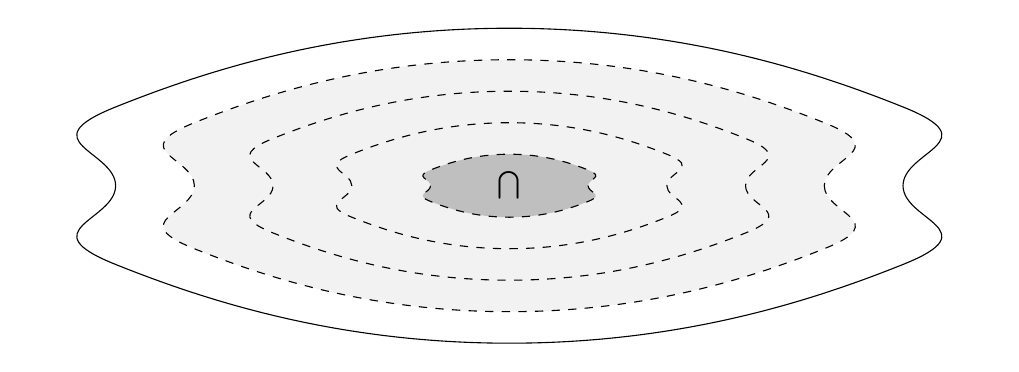
\begin{tikzpicture}
        \pic at (0, 0) {longspace};
        \foreach \i in {.8, .6, .4}{
            \pic[scale=\i, every path/.style={fill=ballfill, dashed}] at (0, 0)
                {longspace};
        }
        \pic[scale=.2, every path/.style={fill=lightgray, dashed}] at (0, 0)
            {longspace} node {$ \bigcap $};
    \end{tikzpicture}
    \captionof{figure}{We consider the intersection of open sets using the
        smallest open ball $ B(x, \epsilon) $.}
\end{theorem}
\begin{theorem}{Summary of \texorpdfstring{$ T_d $}{Open Set} Properties}
        {summary-open-set}
    Let $ (X, d) $ be a metric space, and let $ T_d $ be the topology induced by
    $ d $. Then,
    \setaxiomprefix{T}
    \begin{axioms}
        \item $ \emptyset, X \in T_d $;
        \item For any collection of open sets $ \Lambda \subseteq T_d $,
            $ \bigcup_{\Omega \in \Lambda} \Omega \in T_d $ is open
            (\cref{theorem:open-union-open});\label{axiom:open-union-open}
        \item For any finite collection of open sets $ \Omega_1, \ldots,
            \Omega_N \in T_d $, $ \bigcap_{i=1}^N \Omega_i \in T_d $ is open
            (\cref{theorem:open-intersection-open}).
    \end{axioms}
\end{theorem}

\lecture{Lecture VI}{Viewer.aspx?id=ed63db50-27cd-4d84-8e60-b093009be8af}{
    Lecture Six continues to cover the topology induced by a metric by deriving
    the corresponding properties of closed sets. We introduce the concept of
    \emph{topological equivalence} as weaker method of determining ``sameness''
    between metric spaces. We finally define the \emph{closure} of a set, and
    prove that the closure is closed.
}{\DTMdisplaydate{2023}{10}{12}{Tuesday}}

\begin{theorem}{Summary of Closed Set Properties}{summary-closed-set}
    We can easily derive a dual of \cref{theorem:summary-open-set} for arbitrary
    and finite collections of \emph{closed} sets.
    \setaxiomprefix{F}
    \begin{axioms}
        \item For any collection of closed sets $ \mathcal{F} $,
            \begin{equation}
                \text{For all } F \in \mathcal{F} \text{, } \underbrace{F^c \in
                T_d}_\mathrm{\Cref{theorem:open-subset-closed-complement}}
                \implies\underbrace{\bigcup_{F \in \mathcal{F}} \left( F^c
                \right) \in T_d}_\mathrm{\Cref{axiom:open-union-open}} \implies
                \bigcap_{F \in \mathcal{F}} F \text { is closed,}
            \end{equation}
            since $ \left(\bigcap_{F \in \mathcal{F}} F\right)^c =
            \bigcup_{F \in \mathcal{F}} \left( F^c \right) \in T_d $ by De
            Morgan's laws.
        \item Similarly, for any finite collection of closed sets $ F_1, \ldots,
            F_N $,
            \begin{equation}
                \left( \bigcup_{i=1}^N F_i \right)^c = \bigcap_{i=1}^N F_i^c \in
                T_d \implies \bigcup_{i=1}^N F_i \text{ is closed.}
            \end{equation}
    \end{axioms}
\end{theorem}
\begin{definition}{Topological Equivalence}{topological-equivalence}
    Let $ d $ and $ d^* $ be metrics on a set $ X $. Then, $ (X, d) $ and $ (X,
    d^*) $ are \emph{(topologically) equivalent} if and only if $ T_d = T_{d^*}
    $; that is, $ d $ and $ d^* $ induce the same topologies.
\end{definition}
\begin{theorem}{Determining Topological Equivalence}{determining-top-eq}
    Let $ X $ be a set and let $ d $ and $ d^* $ be metrics on $ X $. Then, $
    T_d = T_{d^*} $ if and only if there exists a scalar $ \lambda > 0 $ for
    which
    \begin{equation}
        \frac{1}{\lambda} d(x, y) \leq d^*(x, y) \leq \lambda d(x, y)
    \end{equation}
    for all $ x, y \in X $.
\end{theorem}
\begin{example}{\texorpdfstring{$ \mathbb{R}^2 $}{The plane} is topologically
        equivalent under the \texorpdfstring{$ d_1 $, $ d_2 $, and $ d_\infty
        $}{standard} metrics}{plane-top-eq}
    Recall the unit circles $ S_1^2 $ (\cref{fig:d1-unit-circle}), $ S_2^2 $
    (\cref{fig:d2-unit-circle}), and $ S_\infty^2 $
    (\cref{fig:dinf-unit-circle}) from \cref{example:unit-circles}. We claim
    (and give an information demonstration to show) that $ T_{d_1} = T_{d_2} =
    T_{d_\infty} $; that is, $ d_1 $, $ d_2 $, and $ d_\infty $ are
    topologically equivalent by \cref{definition:topological-equivalence}.

    We first consider the set $ S_1^2 \eqcolon \Omega $ in the space $
    \left(\mathbb{R}^2, d_2\right) $. Take a point $ x_0 \in \Omega $ and
    construct the open ball $ B(x_0, \epsilon/2) \subseteq S_1^2 $; such a ball
    can be created by considering an $ \epsilon \coloneq \min\left\{ \epsilon_1,
    \epsilon_2, \epsilon_3, \epsilon_4 \right\} $, where $ \epsilon_i $ for $ i
    = 1, 2, 3, 4 $ are the perpendicular distances from $ x_0 $ to the boundary
    of $ \Omega $ by the $ d_2 $ metric. Then, $ \Omega \in T_{d_2} $.

    Next, consider $ S_2^2 \eqcolon \Lambda $ in the space $ \left(\mathbb{R}^2,
    d_1\right) $. Constructing open balls in $ d_1 $ around the points in $
    \Lambda $ is easier still, since we only need to consider `diamonds' which
    lie entirely within the Euclidean $ d_2 $ unit circle. By covering the
    entire set, we can conclude that $ \Lambda \in T_{d_1} $.

    Intuitively, we can see that the metrics $ d_1 $ and $ d_2 $ induce the same
    topologies; analogous arguments apply for establishing the equivalences to $
    d_\infty $.

    \centering
    \begin{minipage}{.45\linewidth}
        \centering
        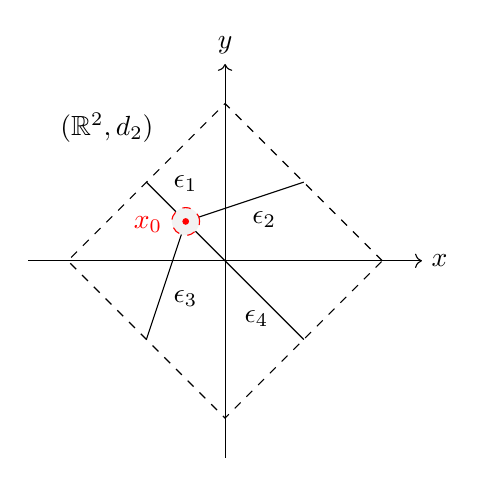
\begin{tikzpicture}
            \coordinate (x0point) at (-.5, .5);
            \draw[->] (-2.5, 0) -- (2.5, 0) node[right] {$x$};
            \draw[->] (0, -2.5) -- (0, 2.5) node[above] {$y$} node[left=1.5cm,
                below=.5cm] {$ (\mathbb{R}^2, d_2) $};
            \node[diamond, dashed, draw, minimum width=4cm, minimum height=4cm]
                {};
            \draw (x0point) -- (-1, 1) node[above, pos=.5, xshift=7pt]
                {$ \epsilon_1 $};
            \draw (x0point) -- (1, 1) node[below, pos=.5, xshift=7pt]
                {$ \epsilon_2 $};
            \draw (x0point) -- (-1, -1) node[below, pos=.5, xshift=7pt]
                {$ \epsilon_3 $};
            \draw (x0point) -- (1, -1) node[below, pos=.6, yshift=-3pt]
                {$ \epsilon_4 $};
            \draw[red, dashed, fill=ballfill] (x0point) circle (5pt);
            \filldraw[red] (x0point) circle (1pt) node[left, red, xshift=-5pt,
                yshift=-1pt] {$ x_0 $};
        \end{tikzpicture}
        \captionof{figure}{Considering the $ d_1 $-defined unit circle $ \Omega
            $ as an open set in the $ \left(\mathbb{R}^2, d_2\right) $ space.}
    \end{minipage}\hfill
    \begin{minipage}{.45\linewidth}
        \centering
        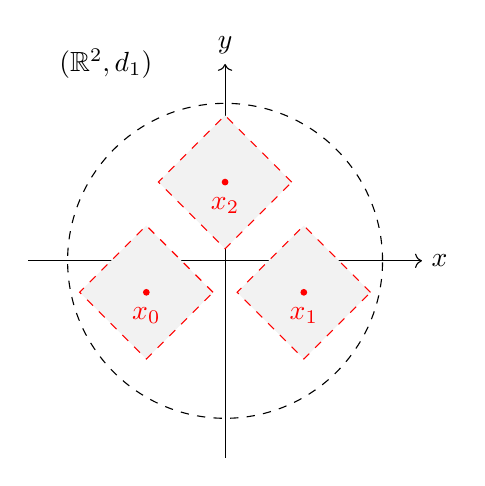
\begin{tikzpicture}
            \coordinate (x0point) at (-1, -.4);
            \coordinate (x1point) at (1, -.4);
            \coordinate (x2point) at (0, 1);
            \draw[->] (-2.5, 0) -- (2.5, 0) node[right] {$x$};
            \draw[->] (0, -2.5) -- (0, 2.5) node[above] {$y$} node[left=.8cm]
                {$ (\mathbb{R}^2, d_1) $};
            \draw[dashed] (0, 0) circle (2cm);
            \foreach \i in {0, 1, 2} {
                \node[diamond, draw, minimum width=1.7cm, minimum height=1.7cm,
                    dashed, red, fill=ballfill] at (x\i point) {};
                \filldraw[red] (x\i point) circle (1pt) node[below, yshift=-2pt]
                    {$ x_\i $};
            }
        \end{tikzpicture}
        \captionof{figure}{Considering the $ d_2 $-defined unit circle $
            \Lambda $ as an open set in the $ \left(\mathbb{R}^2, d_1\right) $
            space.}
    \end{minipage}
\end{example}
\begin{definition}{Closure}{closure}
    Let $ (X, d) $ be a metric space and $ A \subseteq X $. Then the
    \emph{closure} of $ A $, denoted by $ \overline{A} $, is defined to be $
    \overline{A} = A \cup \partial A $.

    \centering
    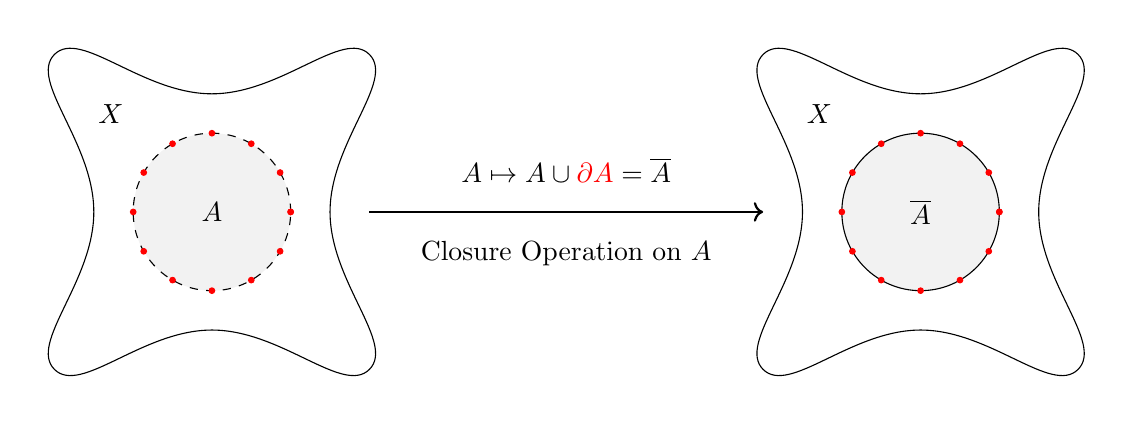
\begin{tikzpicture}
        \coordinate (leftball) at (0, 0);
        \coordinate (rightball) at (9, 0);
        \coordinate (leftbound) at (2, 0);
        \coordinate (rightbound) at (7, 0);
        \pic at (leftball) {squarespace};
        \draw[fill=ballfill, dashed] (leftball) circle[radius=1] node {$ A $}
            node [above left=1cm] {$ X $};
        \pic at (rightball) {squarespace};
        \draw[fill=ballfill] (rightball) circle[radius=1] node
            {$ \overline{A} $} node [above left=1cm] {$ X $};
        \foreach \i in {0, 30, ..., 360} {
            \filldraw[red] (leftball)++(\i:1cm) circle (1pt);
            \filldraw[red] (rightball)++(\i:1cm) circle (1pt);
        }
        \draw[->, thick] (leftbound) -- (rightbound) node [above, pos=.5,
            yshift=7pt] {$ A \mapsto A \cup {\color{red}\partial A} =
            \overline{A} $} node [below, pos=.5, yshift=-7pt]
            {Closure Operation on $ A $};
    \end{tikzpicture}
    \captionof{figure}{Encapsulating the boundary of an open set $ A $ is the
    most `efficient' way of generating a closed set $ \overline{A} $ with the
    same interior $ A^o $.}
\end{definition}
\begin{theorem}{The closure is closed}{closure-closed}
    For an open set $ A \subseteq X $, the closure $ \overline{A} $ is closed.
    \begin{proof}
        By \cref{theorem:open-subset-closed-complement}, $ \overline{A} $ is
        closed if and only if $ \left(\overline{A}\right)^c $ is open. If $
        \left(\overline{A}\right)^c = \emptyset $, then we are done since the
        empty set is known to be open; thus we assume that $
        \left(\overline{A}\right)^c \neq \emptyset $. To prove the openness of
        this non-empty set, we consider an arbitrary point $ x \in
        \left(\overline{A}\right)^c $ and construct an $ \epsilon > 0 $ such
        that $ B(x, \epsilon) \subseteq \left(\overline{A}\right)^c $.

        Since $ \overline{A} = A \cup \partial A $, $ x \not\in A $ and $ x
        \not\in \partial A $. We can use rules from first-order logic combined
        with De Morgan's laws to negate the definition of a boundary point shown
        in \cref{definition:boundary-points}:
        \begin{align}
            x \in \left(\partial A\right)^c &= \left\{ y \in X \colon \forall
                \epsilon > 0 \, B(y, \epsilon) \cap A \neq \emptyset \land B(y,
                \epsilon) \cap A^c \neq \emptyset \right\}^c \\
            &= \left\{ y \in X \colon \forall \epsilon > 0 \, B(y, \epsilon)
                \cap A = \emptyset \lor B(y, \epsilon) \cap A^c = \emptyset
                \right\} \\
            &= \left\{ y \in X \colon \forall \epsilon > 0 \, B(y, \epsilon)
                \subseteq A^c \lor B(y, \epsilon) \subseteq A \right\}
        \end{align}
        Since $ x \not\in A $, $ B(x, \epsilon) \subseteq A^c $ is the only
        possibility. We also require that $ x \not\in \partial A $, so we need
        to show that there is an $ \epsilon > 0 $ such that $ B(x, \epsilon)
        \cap \partial A = \emptyset $. By way of contradiction, suppose that
        there exists a $ y \in B(x, \epsilon) $ such that $ y \in \partial A $.
        By definition \cref{definition:boundary-points}, for all $ \delta > 0 $,
        \begin{equation}
            B(y, \delta) \cap A \neq \emptyset \text{ and } B(y, \delta) \cap
            A^c \neq \emptyset.
        \end{equation}
        If $ d(x, y) \eqcolon \epsilon^* < \epsilon $, and $ \hat{\epsilon}
        \coloneq \min\left\{ \epsilon^*, \epsilon - \epsilon^* \right\} $, then
        $ B(y, \hat{\epsilon}/2) \subseteq B(x, \epsilon) $. But $ B(y,
        \hat{\epsilon}) \cap A \neq \emptyset $. This is a contradiction: no
        such $ y $ can exist, so $ \left(\overline{A}\right)^c $ is open, and $
        \overline{A} $ is closed.
    \end{proof}
    \centering
    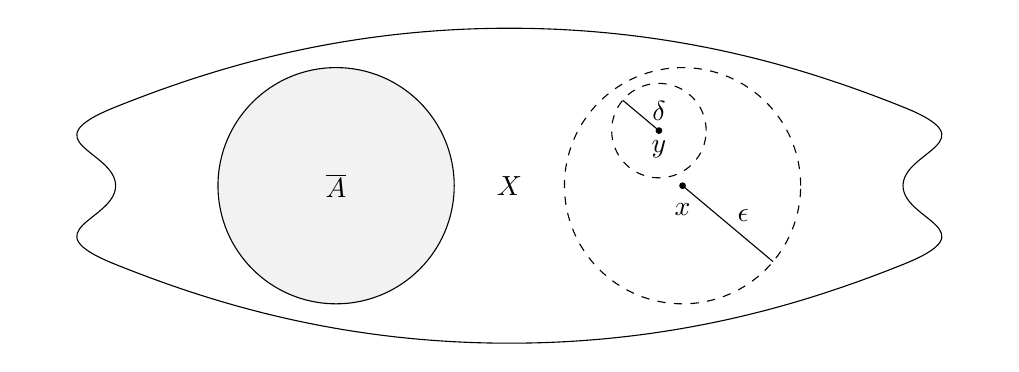
\begin{tikzpicture}
        \coordinate (apos) at (-2.2, 0);
        \coordinate (xpos) at (2.2, 0);
        \coordinate (ypos) at (1.9, .7);
        \pic at (0, 0) {longspace};
        \node at (0, 0) {$ X $};
        \draw[fill=ballfill] (apos) circle (1.5cm) node {$ \overline{A} $};
        \draw[dashed] (xpos) circle (1.5cm);
        \filldraw (xpos) circle (1pt) node[below, yshift=-3pt] {$ x $};
        \draw (xpos) -- ++(320:1.5cm) node[right, pos=.5, yshift=3pt]
            {$ \epsilon $};
        \draw[dashed] (ypos) circle (.6cm);
        \filldraw (ypos) circle (1pt) node[below] {$ y $} node[above]
            {$ \delta $};
        \draw (ypos) -- ++(140:.6cm);
    \end{tikzpicture}
    \captionof{figure}{The open ball $ B(x, \epsilon) $ lies entirely within the
        complement of the closure of $ A $, within which $ B(y, \delta) $ is
        nested.}
\end{theorem}

\lecture{Lecture VII}{}{
    Lecture Seven demonstrates that a space is closed if and only if it is equal
    to its own closure, and moves to introduce the topic of
    limit/accumulation/cluster points whilst proving some useful related
    properties.
}{}

\begin{theorem}{Relationships between a closed set and its
        closure}{closed-set-closure}
    If $ A \subseteq X $ is closed, then $ A = \overline{A} $; if $ A =
    \overline{A} $, then $ A $ is closed. That is, $ A $ is closed if and only
    if $ A = \overline{A} $.
    \begin{proof}
        \iffforward If $ A = \overline{A} $, then $ \overline{A} $ is closed by
        \cref{theorem:closure-closed}. Thus $ A $ is closed.

        \iffbackward If $ A $ is closed, then $ \overline{A} = A \cup \partial A
        $ by \cref{definition:closure}. By
        \cref{definition:open-closed-clopen-sets}, $ \overline{A} = \partial A
        \cup \overline{A} = A $.
    \end{proof}
\end{theorem}
\begin{definition}{Limit/Accumulation/Cluster Points}{limit-points}
    \begin{minipage}{.6\linewidth}
        Let $ (X, d) $ be a metric space, and $ A \subseteq X $. A \emph{limit
        point} $ y \in X $ of $ A $ is an element of $ X $ for which
        \begin{equation}
            \left[ B(y, \epsilon) \setminus \{y\} \right] \cap A \neq \emptyset
            \text{ for all } \epsilon > 0.
        \end{equation}
        The \emph{derived set} of $ A $ is denoted $ A^\prime $, and is defined
        to be the set of all limit points of $ A $. Equivalently (in the context
        of metric spaces, but not the more general topological spaces), we can
        say that $ y \in X $ is a limit point of $ A $ if, for any $ \epsilon >
        0 $, the intersection $ B(y, \epsilon) \cap A $ contains infinitely many
        points of $ A $. Limit points are sometimes called \emph{accumulation
        points} or \emph{cluster points}.
    \end{minipage}\hfill
    \begin{minipage}{.35\linewidth}
        \centering
        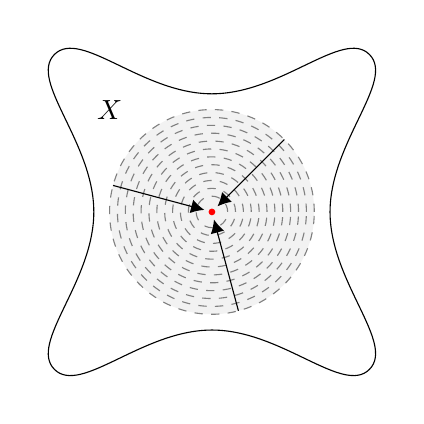
\begin{tikzpicture}
            \pic at (0, 0) {squarespace};
            \node at (-1.3, 1.3) {$ X $};
            \fill[ballfill] (0, 0) circle (1.3cm);
            \foreach \radius in {1.3, 1.2, ..., .1}
                \draw[dashed, gray] (0, 0) circle (\radius cm);
            \filldraw[red] (0, 0) circle (1pt);
            \foreach \angle in {45, 165, 285}
                \draw[-{Latex[width=5pt]}] (\angle:1.3cm) -- (\angle:.1cm);
        \end{tikzpicture}
        \captionof{figure}{As the open balls contract \emph{ad infinitum}, we
            can still find non-centroid points of $ A $.}
    \end{minipage}
\end{definition}
\begin{theorem}{The closure of a set is the union of the base set and its
        derived set}{closure-limit-union}
    For a set $ A \subseteq X $, $ \overline{A} = A \cup A^\prime $.
    \begin{proof}
        If $ A $ is closed, then the result is immediate: $ \overline{A} = A $
        (by \cref{theorem:closed-set-closure}), so $ A^\prime \subseteq A =
        \overline{A} $. Thus, we assume that $ A $ is open. If $ A^\prime =
        \emptyset $, then $ A^\prime \subseteq \overline{A} $, since $ A $ has
        no limit points; therefore, we also assume that $ A $ is non-empty. We
        will show the equality $ \overline{A} = A \cup A^\prime $ for an open
        non-empty set $ A $ through the principle of double-inclusion.

        \iffforward Without loss of generality, suppose that $ y $ is such that
        $ y \in \partial A $ and $ y \not\in A $. For any choice of $ \epsilon >
        0 $, we know that $ B(y, \epsilon) \cap A \neq \emptyset $. Since $ y
        \not\in A $, there exists a $ y^\prime \neq y \in A, B(y, \epsilon) $.
        This is consistent with \cref{definition:limit-points}. Thus, $ y $ is a
        limit point, so $ A^\prime \subseteq \overline{A} $ and $ A \cup
        A^\prime \subseteq \overline{A} $.

        \iffbackward Given that $ A $ is not closed, there exists a $ y \in
        A^\prime $ such that $ y \not\in A $. Take $ \epsilon > 0 $ and note
        that $ B(y, \epsilon) \cap A \neq \emptyset $ and $ B(y, \epsilon) \cap
        A^c \neq \emptyset $. Thus, by \cref{definition:boundary-points}, $ y $
        is a boundary point. We now unravel the definitions:
        \begin{alignat}{2}
            A \text{ is closed} &\iff \partial A \subseteq A
                &&\mathrm{[\Cref{definition:open-closed-clopen-sets}]} \\
            &\iff A^c \text{ is open}
                &&\mathrm{[\Cref{theorem:open-subset-closed-complement}]}%
                \label{eqn:closure-limit-union-open} \\
            &\iff A^c \cap \partial \left( A^c \right) = \emptyset
                &&\mathrm{[\Cref{definition:open-closed-clopen-sets}]} \\
            &\iff A^c \cap \partial A = \emptyset
                &&\mathrm{[\Crefrange{eqn:boundary-complement-boundary-first}%
                    {eqn:boundary-complement-boundary-last}]} \\
            &\iff \forall x \in A^c,\, \exists \epsilon > 0 \text{ s.t. }
                B(x, \epsilon) \subseteq A^c\quad
                &&\mathrm{[\Cref{eqn:closure-limit-union-open}]} \\
            &\iff A = \overline{A} \\
            &\iff A \supseteq A^\prime
        \end{alignat}
        Hence, $ \overline{A} = A \cup \partial A = A \cup A^\prime $ for any
        $ A \subseteq X $.
    \end{proof}
\end{theorem}
\begin{definition}{Topological Interpretation of Closure}{topological-closure}
    Let $ (X, d) $ be a metric space, and $ A \subseteq X $. Then,
    \begin{equation}
        \overline{A} = \bigcap_{F \in \mathcal{F}} F,
    \end{equation}
    where $ \mathcal{F} $ is the collection of all open supersets of $ A $. This
    means that $ \overline{A} $ is the smallest closed superset of $ A $.
\end{definition}
\begin{definition}{Density}{density}
    Let $ (X, d) $ be a metric space and $ A \subseteq X $. Then $ A $ is said
    to be \emph{dense} in $ X $ if and only if $ \overline{A} = X $.
    Alternatively---but equivalently---for any $ x \in X $ and any $ \epsilon >
    0 $, there exists an $ a \in A $ such that $ d(x, a) < \epsilon $.
\end{definition}

\lecture{Lecture VIII}{Sessions/List.aspx\#folderID="072999e9-f3bc-4486-98af-%
        b0a000d51b97"}{
    Lecture Eight gives the definition of a \emph{sequence} in a metric space,
    and motivates the study of various properties thereof, such as
    \emph{convergence}. Some examples are provided, with familiar concepts from
    Real Analysis being recast into the more abstract setting of metric and
    topological spaces.
}{\DTMdisplaydate{2023}{10}{19}{Thursday}}

\begin{definition}{Sequence}{sequence}
    A \emph{sequence} in a metric space $ (X, d) $ is an element of $
    X^\mathbb{N} $, where any element $ x \in X^\mathbb{N} $ can be written as a
    countable set $ x = \left\{ x_1, \ldots, x_n, \ldots \right\} $, such that
    $ x_i \in X $ for all $ i \in \mathbb{N} $. Such a sequence is denoted
    \begin{equation}
        \left( x_n \right)_{n \in \mathbb{N}} \text{ or }
        \left( x_n \right)_{n=1}^\infty.
    \end{equation}
\end{definition}
\begin{definition}{Convergence of Sequences (by the Metric)}
        {sequence-convergence-metric}
    Let $ \left( x_n \right)_{n \in \mathbb{N}} $ be a sequence in $ (X, d) $.
    Then, $ \left( x_n \right)_{n \in \mathbb{N}} $ \emph{converges} to $ x \in
    X $ if and only if
    \begin{equation}
        \text{For all } \epsilon > 0 \text{, there exists an } N=N(\epsilon)
        \text{ such that } d(x_n, x) < \epsilon \text{ for all } n > N.
    \end{equation}
    If this is the case, we write $ x_n \to x $ (as $ n \to \infty $), and the $
    x $ is \emph{the} (unique) limit of $ \left(x_n\right)_{n \in \mathbb{N}} $.
    If no such $ x $ exists, then $ \left(x_n\right)_{n \in \mathbb{N}} $ is
    \emph{divergent}.

    \centering
    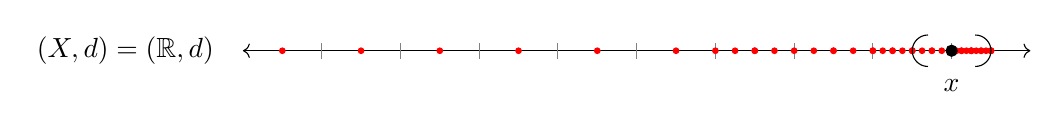
\begin{tikzpicture}
        \draw[<->] (-5, 0) -- (5, 0) node[pos=0, left, xshift=-7pt] {$ (X, d) =
            (\mathbb{R}, d) $}; % Number line and markings
        \foreach \i in {-4, ..., 4} \draw[gray] (\i, -.1) -- (\i, .1);

        \foreach \i in {-4.5, -3.5, ..., 4.5}
            \filldraw[red] (\i, 0) circle (1pt); % Spacing: 1, Start: -4.5

        \foreach \i in {1, 1.25, ..., 4.5}
            \filldraw[red] (\i, 0) circle (1pt); % Spacing: 0.25, Start: 1

        \foreach \i in {3, 3.125, ..., 4.5}
            \filldraw[red] (\i, 0) circle (1pt); % Spacing: 0.125, Start: 3

        \foreach \i in {4, 4.0625, ..., 4.5}
            \filldraw[red] (\i, 0) circle (1pt); % Spacing: 0.0625, Start: 4

        \filldraw (4, 0) circle (2pt) node[below=7pt] {$ x $};

        \draw (3.7, .2) arc[start angle=90, end angle=270, radius=.2]; % L. arc
        \draw (4.3, .2) arc[start angle=90, end angle=-90, radius=.2]; % R. arc
    \end{tikzpicture}
    \captionof{figure}{A sequence in $ (\mathbb{R}, d) $, where $ d $ is the
        standard metric, converging to an $ x \in \mathbb{R} $. The \emph{zone
        of convergence} $ (x-\epsilon, x+\epsilon) $ is denoted with parentheses
        about $ x $.}
\end{definition}
\begin{definition}{Convergence of Sequences (by the Open Balls)}
        {sequence-convergence-balls}
    An equivalent notion of convergence can be expressed in terms of open balls,
    such that the tail of the sequence exists in the open ball centered at the
    limit. Let $ \left( x_n \right)_{n \in \mathbb{N}} $ be a sequence in $ (X,
    d) $. Then, $ \left( x_n \right)_{n \in \mathbb{N}} $ \emph{converges} to $
    x \in X $ if and only if
    \begin{equation}
        \forall \epsilon > 0\, \exists N > 0 \text{ such that } x_n \in B(x,
        \epsilon)\, \forall n > N.
    \end{equation}
    That is, for any given $ \epsilon > 0 $, we must find an index $ N $ for the
    sequence $ (x_n)_{n \in \mathbb{N}} $ after which all points $ x_i\,\, (i >
    N) $ exist within the open ball $ B(x, \epsilon) $. If this holds, then the
    sequence $ (x_n) $ converges to the centre of the open ball $ x $.

    \centering
    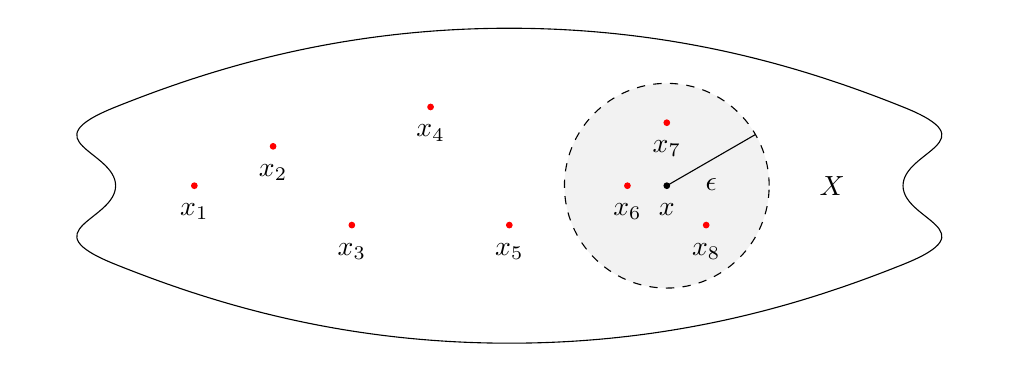
\begin{tikzpicture}
        \coordinate (ballcentre) at (2, 0);
        \pic at (0, 0) {longspace};
        \draw[fill=ballfill, dashed] (ballcentre) circle (1.3cm);
        \filldraw (ballcentre) circle (1pt) node[below, yshift=-3pt] {$ x $};
        \draw (ballcentre) -- ++(30:1.3cm) node[pos=.5, below, yshift=-3pt]
            {$ \epsilon $};
        \node at (4.1, 0) {$ X $};

        \begin{scope}[every path/.style={red}, every node/.style={black, below,
                yshift=-3pt}]
            \filldraw (-4, 0) circle (1pt) node {$ x_1 $};
            \filldraw (-3, .5) circle (1pt) node {$ x_2 $};
            \filldraw (-2, -.5) circle (1pt) node {$ x_3 $};
            \filldraw (-1, 1) circle (1pt) node {$ x_4 $};
            \filldraw (0, -.5) circle (1pt) node {$ x_5 $};
            \filldraw (1.5, 0) circle (1pt) node {$ x_6 $};
            \filldraw (2, .8) circle (1pt) node {$ x_7 $};
            \filldraw (2.5, -.5) circle (1pt) node {$ x_8 $};
        \end{scope}
    \end{tikzpicture}
    \captionof{figure}{A sequence converging within the bounds of an arbitrarily
    sized open ball centred at the limit. In this example, $ N = 5 $, since all
    sequence points $ x_6, x_7, x_8, \ldots $ belong to the pictured open ball.}
\end{definition}
\begin{definition}{Convergence of Sequences (by the convergence of a real
        sequence)}{sequence-convergence-real}
    We can also use results from Real Analysis to consider the real sequence
    generated by the distances between each point in the space and the proposed
    limit $ x $. For a sequence $ \left( x_n \right)_{n \in \mathbb{N}} $ in a
    metric space $ (X, d) $,
    \begin{equation}
        \lim_{n \to \infty} x_n = x \iff \lim_{n \to \infty} d(x_n, x) \to 0.
    \end{equation}
\end{definition}
\begin{theorem}{Convergences of Real-Dimensional Vector
        Spaces}{vector-space-convergence}
    In $ \mathbb{R}^k $ with any $ d_1 $, $ d_2 $, or $ d_\infty $ metrics,
    \emph{overall convergence is equivalent to simultaneous component-wise
    convergence}. That is, for $ \vec{x}_n \in \mathbb{R}^k $ with $ n \in
    \mathbb{N} $,
    \begin{equation}
        \lim_{n \to \infty} \vec{x}_n \to \vec{x} \iff
        \lim_{n \to \infty} x_i^{(n)} \to x_i \text{ for each } i \in \left\{1,
        \ldots, k \right\}.
    \end{equation}
    Note that $ \vec{x} = (x_1, \ldots, x_k) $ denotes a general
    vector/candidate limit, and $ \vec{x}_n = \left(x_1^{(n)}, \ldots,
    x_k^{(n)}\right) $ denotes a $ k $-dimensional vector in the sequence at
    index $ n $. For this demonstration, we will consider the specific case of
    $ \left(\mathbb{R}^k, d_\infty\right) $.
    \begin{proof}
        \iffforward Suppose that $ \vec{x}_n \to \vec{x} $ as $ n \to \infty $.
        We want to show that, for each $ i \in \left\{ 1, \ldots, k \right\} $,
        the components converge such that $ x_i^{(n)} \to x_i $ as $ n \to
        \infty $. Let $ \epsilon > 0 $ be given. Since $ \lim_{n \to \infty}
        \vec{x}_n = \vec{x} $, there exists an $ N(\epsilon) > 0 $ such that
        $ d_\infty(\vec{x}_n, \vec{x}) < \epsilon $ for all $ n > N $. By
        recalling the mapping definition of $ d_\infty $ from
        \cref{definition:canon-metrics}, we can derive that
        \begin{equation}
            \max_{1 \leq i \leq k} \left\vert x_i^{(n)} - x_i \right\vert <
            \epsilon \text{ for all } n > N.
        \end{equation}
        By the nature of the maximum function, we can generalise this inequality
        to all choices of $ i \in \left\{ 1, \ldots, k \right\} $:
        \begin{equation}
            \left\vert x_i^{(n)} - x_i \right\vert < \epsilon \text{ for all } n
            > N \text{ for all } i \in \left\{1, \ldots, k \right\}.
        \end{equation}
        We can immediately arrive at the desired limit for the real sequence: $
        \lim_{n \to \infty} x_i^{(n)} = x_i $ for all $ i \in \left\{ 1, \ldots,
        k \right\} $.

        \iffbackward Now suppose that $ \lim_{n \to \infty} x_i^{(n)} = x_i $
        for all $ i \in \left\{ 1, \ldots, k \right\} $, and let $ \epsilon > 0
        $ be given. Then, for any suitable choice of $ i $, there exists an $
        N_i(\epsilon) > 0 $ such that $ \left\vert x_i^{(n)} - x_i \right\vert <
        \epsilon $ for all $ n > N_i $.
        \begin{equation*}
            \renewcommand\arraystretch{1.5}
            \begin{matrix}
                \vec{x}_1 & \vline & x_1^{(1)} & x_2^{(1)} & x_3^{(1)} & \ldots
                    & x_k^{(1)} \\
                \vec{x}_2 & \vline & x_1^{(2)} & x_2^{(2)} & x_3^{(2)} & \ldots
                    & x_k^{(2)} \\
                \vec{x}_3 & \vline & x_1^{(3)} & x_2^{(3)} & x_3^{(3)} & \ldots
                    & x_k^{(3)} \\
                \vdots & \vline & \vdots & \vdots & \vdots & \ddots & \vdots \\
                \vdots & \vline & \multirow{2}{*}{$ \begin{cases} ~~N_1 \\
                    ~~~\vdots \end{cases} $} & \big\downarrow & N_3 &
                    \big\downarrow & N_k & \multirow{2}{*}{\hspace{-1ex}
                    $ \begin{rcases} \vphantom{~}\\\vphantom{~}\end{rcases} $}
                    \\ % What the fuck?
                \vdots & \vline & & N_2 & \vdots & N_j & \vdots \\
                & & \multicolumn{6}{c}{\text{Zones of Convergence}}
            \end{matrix}
        \end{equation*}
    \end{proof}
\end{theorem}
\end{document}

